\section{Core functions}

Here we will describe the core parts of the code defining the signal model and the probability functions used
for the inference. These assume that the data comprises a number of calibrated narrow-band complex-heteroyned time
series'. These time series data streams can be from different detectors, and/or at different heterodyne
frequencies. For example you could have a pair of times series from both the LIGO Hanford (H1) and LIGO
Livingston (L1) detectors, with one produced with a heterodyne at twice the rotation frequency of a known
pulsar and the other produced with a heterodyne at the rotation frequency.

\subsection{The signal model}\label{sec:model}

Our code assumes that the electromagnetically observed rotational phase evolution of a pulsar is represented by its Taylor expansion
\begin{equation}
\phi(t) = 2\pi\left(fT(t) + \frac{1}{2}\dot{f}T(t)^2 + \frac{1}{6}\ddot{f}T(t)^3 \ldots \right)
\end{equation}
where $T$ is the time, corrected to an inertial reference frame (the solar system barycentre
for isolated pulsars, or the binary system barycentre for pulsars in binaries or multiple component systems), and the $f$'s give
the observed rotation frequency and its time derivatives. The value of $T = (t+\tau(t)-t_0)$ where $t$ is the
time at a detector, $\tau(t)$ is the time dependent correction to the inertial frame and $t_0$ is the epoch.
The code can accept frequency derivatives of any order. We assume the
calibrated detector data, $d(t)$, has been heterodyned such that
\begin{equation}
B'(t) = d(t)e^{-i\Phi_{i,\text{het}}(t)},
\end{equation}
where $\Phi_{i,\text{het}}(t)$ is the phase evolution for a given data stream $i$, and we produce $B(t)$ by
low-pass filtering and resampling (via averaging) values of $B'(t)$.

Under the standard assumption that the general theory of relativity (GR) is correct the code uses the form of
the signal model defined in \citet{2015arXiv150105832J}, which, when heterodyned and assuming low-pass
filtering, gives a signal at a pulsar's rotation frequency (where $\Phi_{1,{\text{het}}}(t) = \phi(t)$) of
\begin{widetext}
\begin{equation}\label{eq:hf}
h_f(t) =  e^{i\Delta\phi_1(t)}\left(-\frac{C_{21}}{4}F_{+}(\psi,t)\sin{\iota}\cos{\iota}\,e^{i\Phi_{21}^C} +
i\frac{C_{21}}{4}F_{\times}(\psi,t)\sin{\iota}\,e^{i\Phi_{21}^C} \right)
\end{equation}
and at twice the pulsar's rotation frequency (where $\Phi_{2,{\text{het}}}(t) = 2\phi(t)$) of
\begin{equation}\label{eq:h2f}
h_{2f}(t) =  e^{i\Delta\phi_2(t)}\left(-\frac{C_{22}}{2}F_{+}(\psi,t)[1+\cos{}^2\iota]e^{i\Phi_{22}^C} +
iC_{22}F_{\times}(\psi,t)\cos{\iota}\,e^{i\Phi_{22}^C} \right).
\end{equation}
\end{widetext}
The $F_{+}$ and $F_{\times}$ values are the detector dependent antenna patterns \citep[see, e.g., equation~\ref{eq:antenna}, taken from][]{1998PhRvD..58f3001J},
which are a function of the
detector position, source sky position and source polarisation angle $\psi$. The $C_{21}$, $C_{22}$,
$\Phi_{21}^C$ and $\Phi_{22}^C$ values are convenient ways of representing the waveform in terms of an
amplitude and phase of the signal for the $l=2$, $m=1$ harmonic and $l=m=2$ harmonic respectively. The
$\Delta\phi(t)$ values represent any time dependent phase deviation between the phase used in the heterodyne
and the true signal phase \citep[which does not necessarily have to precisely follow the electromagnetically observed rotational phase, see discussions in, e.g.,][]{2008ApJ...683L..45A}, so
$\Delta\phi_1(t) = (\phi_{1,{\text{true}}}(t)-\Phi_{1,{\text{het}}}(t))$ and $\Delta\phi_2(t) = (\phi_{2,{\text{true}}}(t)-\Phi_{2,{\text{het}}}(t))$. More generally,
for emission at an arbitrary scaling of the rotation frequency, $\mathcal{K}$ (where $\Phi_{\mathcal{K},{\text{het}}}(t) = \mathcal{K}\phi(t)$), an even more generic signal model (still assuming GR is correct) would be
\begin{equation}\label{eq:hkf}
h_{\mathcal{K}f}(t) =  \frac{e^{i\Delta\phi_{\mathcal{K}}(t)}}{2}\left(H_+F_{+}(\psi,t)e^{i\Phi_0} +
iH_{\times}F_{\times}(\psi,t)e^{i\Phi_{0}} \right),
\end{equation}
where $H_+$ and $H_{\times}$ are the amplitude components for the `$+$' and `$\times$' polarisations, and $\Phi_0$ is the signal's initial phase.

To calculate the $\Delta\phi_{\mathcal{K}}$ values using up to the $(n-1)^{\text{th}}$ frequency derivative, and try to avoid numerical overflow issues when dealing
with large phases, we use
\begin{widetext}
\begin{equation}\label{eq:deltaphi}
\Delta\phi_{\mathcal{K}}(t) = 2\pi \mathcal{K} \sum_{k=1}^n \left( \frac{\left(f^{(k-1)}_{{\text{true}}} - f^{(k-1)}_{{\text{het}}}\right)}{k!}(t+\delta t_{\text{het}})^k + \frac{f^{(k-1)}_{{\text{true}}}}{k!} 
\sum_{i=0}^{i<k} \left(\begin{array}{c}k \\ i\end{array} \right) (\delta t_{\text{true}}-\delta t_{\text{het}})^{k-i} (t+\delta t_{\text{het}})^i \right),
\end{equation}
\end{widetext}
where $f^{(n)}$ is the $n^{\text{th}}$ frequency derivative (for both the `true' and `het' values these will be those prior to scaling with $\mathcal{K}$ for
a given signal model), and $\delta t$ is the combination of any solar system barycentring and binary system barycentring time delays.

By default the code assumes emission just from the $l=m=2$ mode, i.e.\ there is only a signal at twice the
rotation frequency. In this case $C_{22}$ and $\Phi_{22}^C$ can be related to the more familiar physical
$h_0$ and $\phi_0$ values via $h_0 = -2C_{22}$ \citep[where the minus sign maintains consistency of equation~\ref{eq:h2f} with the form given in][]{1998PhRvD..58f3001J} and pulsar rotational 
phase $\phi_0 = \Phi_{22}^C/2$. For the more general case the
relations between the waveform amplitude and phase parameters and physical source parameters are given in
\citet{2015arXiv150105832J} and \citet{2015MNRAS.453.4399P}. In general, for previous searches we have often assumed that we track the true
signal phase perfectly with the heterodyne, and as such $\Delta\phi_{\mathcal{K}}(t) = 0$. In such cases the only time
varying components of the signal are the antenna pattern functions, which allows great speed increases in the
signal generation and likelihood calculations (see \S\ref{sec:fastlike}).

\subsubsection{General tensor-vector-scalar signal model}

A more generic {\it heterodyned} model, assuming gravity is described by an arbitrary metric theory, but not necessarily GR, is given by
\citep[see, e.g.][]{2015PhRvD..91h2002I,MaxCWpolariations}
\begin{widetext}
 \begin{equation}\label{eq:hnongr}
    h_{\mathcal{K}f}^{\text{tvs}}(t) =  \frac{e^{i\Delta\phi_{\mathcal{K}}(t)}}{2}\left[ e^{i\Phi_{\text{t}}}\left(F_+H_+ + F_{\times}H_{\times}e^{i\psi_{\text{t}}}\right)
    + e^{i\Phi_{\text{v}}}\left(F_{\text{x}}H_{\text{x}} + F_{\text{y}}H_{\text{y}}e^{\psi_{\text{v}}}\right) + e^{i\Phi_{\text{s}}}\left(F_{\text{b}}H_{\text{b}} + F_{\text{l}}H_{\text{l}}e^{i\psi_{\text{s}}} \right)\right],
 \end{equation}
\end{widetext}
where $H_{p}$ (for $p \in \{+,\times,\text{x},\text{y},\text{b},\text{l}\}$) are the amplitudes for the tensor (`$+$' and `$\times$'), vector (`x' and `y'),
and scalar (`b' and `l') \gw amplitude components, $F_{p}$ are their associate time dependent antenna responses
\citep[see, e.g.][]{2009PhRvD..79h2002N,2012PhRvD..85d3005B,2015PhRvD..91h2002I}, and $\Phi_{\text{t,v,s}}$ and $\psi_{\text{t,v,s}}$ are angles related to the initial
phase of, and rotation within, the tensor, vector and scalar components. For a standard \gw interferometer the two scalar components are entirely
degenerate, and as such only one of them needs to be defined \citep[e.g., only the `b' mode is used in Equation~19 of][]{MaxCWpolariations}. 
When searching for a generic signal such as this the orientation of the wave-frame (given by $\psi$ and $\iota$) used to define the polarisation modes is arbitrary:
one is free to pick any right-handed frame one wants and define the modes there, but we usually make a choice that we know simplifies things for a given signal
(e.g.\ we align the z-axis with the direction of propagation, and/or we align the x-and-y-axes with the detector arms). Hence, for a generic search, we are free to
arbitrarily set our frame such that $\psi=0$ and the values $F_{p}$ given in equation~\ref{eq:hnongr} can be defined by, e.g., equations~24--29 of
\citet{2015PhRvD..91h2002I}. However, when we have a specific prediction of what a given waveform should look like, it is always in a {\it particular} frame. By
convention, this is usually a frame in which the x-axis is aligned with the line of nodes (though the convention is not universal). In other words, if a theory
predicts certain amounts of polarisation with some specific phase evolution (say, that given by GR) then that is a frame dependent statement, and $\psi$ in
required to orient the model frame accordingly. In such a case \citep[e.g., GR or some other theory such as G4v in][]{2015arXiv150304866M} antenna patterns from
equations~30--35 (and $\psi_{\text{t}}$ and $\psi_{\text{v}}$ from equations 46--47, and 49--50, for GR and G4v respectively) of \citet{2015PhRvD..91h2002I}
would be required.

\subsection{The likelihood functions}\label{sec:likelihood}

Our code can make use of two different likelihood functions. The default is a
Student's {\it t}-likelihood function in which it is assumed that the standard deviation of the noise in the
data is unknown, but can be marginalised over. A Gaussian likelihood function can also be used, for
which the code can either take in estimates of the noise standard deviation at each data point, or calculate
these internally based on stationary stretches of data. For the Student's {\it t}-likelihood function, and if
calculating noise standard deviations for the Gaussian likelihood function internally, the code needs to break
up the data into chunks that have characteristics of being from the same Gaussian noise distribution. The method for doing this is
given in \S\ref{sec:splitting}.

\subsubsection{Student's {\it t}-likelihood}\label{sec:stlikelihood}

A full derivation of the Student's {\it t}-likelihood function \citep[see, e.g.,][]{2005PhRvD..72j2002D} is given
in Appendix~\ref{app:likelihood}, but the final form of the joint likelihood (and its natural logarithm,
which is actually used within the code to maintain precision) for multiple detectors and data streams is
given by
\begin{widetext}
\begin{align}\label{eq:stlikelihood}
p(\mathbf{B}|\vec{\theta}) &= \prod_{i=1}^{N_{\text{dets}}} \prod_{j=1}^{N_{\text{s}}} \prod_{k=1}^{M_{i,j}}
\frac{(m_{i,j,k}-1)!}{2\pi^{m_{i,j,k}}}
\left(\sum_{n=n_{i,j,0}}^{n_{i,j,0}+(m_{i,j,k}-1)} |B_{i,j,n}-y(\vec{\theta})_{i,j,n}|^2\right)^{-m_{i,j,k}},
\nonumber \\
\ln{p(\mathbf{B}|\vec{\theta})} &= \sum_{i=1}^{N_{\text{dets}}} \sum_{j=1}^{N_{\text{s}}}
\sum_{k=1}^{M_{i,j}} \left( \mathcal{A}_{i,j,k} - m_{i,j,k}\ln{
\left\{\sum_{n=n_{i,j,0}}^{n_{i,j,0}+(m_{i,j,k}-1)} |B_{i,j,n}-y(\vec{\theta})_{i,j,n}|^2\right\}}
\right),
\end{align}
\end{widetext}
where $N_{\text{dets}}$ is the number of detectors used, $N_{\text{s}}$ is the number of data streams (e.g.,
heterodyned data from both the rotation frequency and twice the rotation frequency) per detector, $M_{i,j}$ is
the total number of independent data chunks for detector $i$ and data stream $j$ with lengths $m_{i,j,k}$, and
$n_{i,j,0} = \sum_{l=1}^{k} 1+m_{i,j,l-1}$ (with $m_{i,j,0} = 0$) being the index of the first data point in
each chunk. The signal model $y(\vec{\theta})$ is that given by Eqns.~\ref{eq:hf} and/or \ref{eq:h2f} (or Eqn.~\ref{eq:hkf})
depending on which data streams are being analysed. For notational convenience we have made the substitution
$\mathcal{A}_{i,j,k} = \ln{\left([m_{i,j,k}-1]!\right)} - \ln{2} - m_{i,j,k}\ln{\pi}$.

\subsubsection{Gaussian likelihood}\label{sec:glikelihood}

The Gaussian likelihood, and its natural logarithm, are similarly given by
\begin{widetext}
\begin{align}\label{eq:gausslikelihood}
p(\mathbf{B}|\vec{\theta}) &= \prod_{i=1}^{N_{\text{dets}}} \prod_{j=1}^{N_{\text{s}}} \prod_{k=1}^{L_{i,j}}
\frac{1}{2\pi\sigma_{i,j,k}^2}\exp{\left(-\frac{|B_{i,j,k}-y(\vec{\theta})_{i,j,k}|^2}{2\sigma_{i,j,k}^2}
\right)}, \nonumber \\
\ln{p(\mathbf{B}|\vec{\theta})} &= \sum_{i=1}^{N_{\text{dets}}} \sum_{j=1}^{N_{\text{s}}}
\sum_{k=1}^{L_{i,j}} \left(\mathcal{B}_{i,j,k} -
\left[\frac{|B_{i,j,k}-y(\vec{\theta})_{i,j,k}|^2}{2\sigma_{i,j,k}^2 } \right] \right)
\end{align}
\end{widetext}
where $L_{i,j}$ is the length of each dataset and $\mathcal{B}_{i,j,k} = -\ln{(2\pi\sigma_{i,j,k}^2)}$. Note
that normalisation factor reflects the fact that exponential is already the product of the real and imaginary data components.

\subsubsection{The null likelihood}\label{sec:nulllike}

As we will most often want to perform model comparison for the signal model against one for which the data just contains
noise (the null hypothesis in this case) we can define the null likelihoods for both of the above likelihoods
by setting $y(\vec{\theta}) = 0$, giving
\begin{align}\label{eq:nulllike}
\ln{p(\mathbf{B}|y=0)} &= \sum_{i=1}^{N_{\text{dets}}} \sum_{j=1}^{N_{\text{s}}}
\sum_{k=1}^{M_{i,j}} \Bigg( \mathcal{A}_{i,j,k} - \nonumber \\
&m_{i,j,k}\ln{
\left\{\sum_{n=n_{i,j,0}}^{n_{i,j,0}+(m_{i,j,k}-1)} |B_{i,j,n}|^2\right\}}
\Bigg),
\end{align}
for the Student's {\it t}-likelihood, and
\begin{equation}
\ln{p(\mathbf{B}|y=0)} = \sum_{i=1}^{N_{\text{dets}}} \sum_{j=1}^{N_{\text{s}}}
\sum_{k=1}^{L_{i,j}} \left(\mathcal{B}_{i,j,k} -
\left[\frac{|B_{i,j,k}|^2}{2\sigma_{i,j,k}^2 } \right] \right)
\end{equation}
for and Gaussian likelihood.

If we were only interested in comparing models calculated using equivalent likelihood functions we could in
general ignore the factors that do not depend on the data or the model, as they would cancel in any odds
ratio. But, in this code we keep them for cases when such a comparison is not performed, e.g.\ if we
want to compared the joint multi-detector likelihood for a signal with the incoherent product of likelihoods
from each detector then we would need these factors to still be present.

\subsubsection{Fast likelihood evaluations}\label{sec:fastlike}

In cases when the only time varying components of the model are the antenna pattern functions (i.e.\ when 
$\Delta \phi_j(t)$ in equation~\ref{eq:hf} or \ref{eq:h2f} is zero) the likelihood
evaluation can be greatly sped-up by pre-calculating the components in the internal summations. For a given sky
position and detector the antenna patterns can be defined by \citep{1998PhRvD..58f3001J}
\begin{align}\label{eq:antenna}
F_+(t,\psi) &= \sin{\zeta}\left[a(t)\cos{2\psi} + b(t)\sin{2\psi}\right], \nonumber \\
F_{\times}(t,\psi) &= \sin{\zeta}\left[b(t)\cos{2\psi} - a(t)\sin{2\psi}\right],
\end{align}
where $\psi$ is the \gw polarisation angle, $\zeta$ is the known angle between the detector arms (generally
$90^{\circ}$), and $a(t)$ and $b(t)$ are the time dependent functions for a given detector position and
source sky location that vary over a sidereal day. These functions can be precomputed at a set of times over
a sidereal day and used, via look-up table interpolation, to give the value at any other time (our code
defaults to calculate $a(t)$ and $b(t)$ at 2880 points over a sidereal day). However, the vast majority of the
speed-up comes from pre-computing summations over the combinations of the data and the $a(t)$ and $b(t)$ functions.
This is described in more detail in Appendix~\ref{app:fle}.

In the case where we want to search over phase evolution parameters that mean that $\Delta\phi_{\mathcal{K}}(t) \ne 0$ in the model then
we cannot perform this pre-summing. However, {\it reduced order quadrature} methods
\citep[e.g.][]{2014PhRvX...4c1006F, 2015PhRvL.114g1104C} may help in these cases. Such a method is implemented in our
code, but will be discussed in a separate paper.

\subsection{The prior functions}\label{sec:priorfuncs}

An important part of any Bayesian inference method is the choice of parameter prior probability functions. Here we describe the prior
functions allowed in the code for any of the required parameters.

Certain parameters are physically not allowed to take negative values, so it is hardcoded that the following parameters
have zero probability below zero: gravitational wave amplitude, $h_0$; $l=m=2$ mass quadrupole moment, $Q_{22}$; the pulsar
distance; the pulsar parallax; the speed of gravitational waves; the projected semi-major axis of a binary orbit; the total
binary system mass; and, the companion mass in a binary system.

There are also other hardcoded priors for waveform amplitudes in two particular cases when searching for emission at both once
and twice the rotation frequency: if searching for a signal from a biaxial star then the two waveform amplitudes, $C_{21}$ and $C_{22}$,
must either both be positive or both be negative; if using the source model then the two amplitudes $I_{21}$ and $I_{31}$, must
have $I_{31} \geqslant I_{21}$.

\subsubsection{Uniform prior}\label{sec:uniformprior}

A parameter can be given a uniform (or flat, or top-hat) prior, in which the probability is constant within a given
range and zero outside that range, i.e.
\begin{equation}
p(x|I) = \begin{cases}
             C & \text{if } x_{\text{min}} < x < x_{\text{max}}, \\
             0 & \text{otherwise},
            \end{cases}
\end{equation}
where for parameter $x$ the upper and lower bounds on the parameter values are $x_{\text{min}}$ and $x_{\text{max}}$. This
prior can be normalised by setting $C = 1/(x_{\text{max}}-x_{\text{min}})$, although within nested sampling the normalisation
is not specifically required. The prior requires a lower and upper bound to allow it to be normalisable and to enable
an initial set of samples to be drawn from it. However, it should be noted that the choice of range will have an
effect on evidences that are calculated.

A histogram of a set of samples produced by the code when drawing from a uniform prior distribution are shown in Figure~\ref{fig:prioruniform},
along with the true prior function.

Some parameters for which the uniform prior is often considered appropriate are angle parameters, such as the $\Phi_{22}^C$ and $\psi$
parameters in Equation~\ref{eq:h2f}, which can be restricted to a specific non-degenerate range \citep[see, e.g., Table~1 in][]{2015MNRAS.453.4399P}. 
In previous gravitational wave pulsar searches, such as \citet{2010ApJ...713..671A,2014ApJ...785..119A} a uniform prior was often used for
the gravitational wave amplitude parameter $h_0$. For those searches the prior upper bound was based on inspection of the data to find a
value that was very large compared to the sensitivity suggested by the data. A uniform prior was used, as opposed to the more
uninformative choice for such a scale parameter of the log-uniform prior (see \S\ref{sec:loguniform}), due to the fact that the main
result was in producing upper limits, and wanting these to be primarily based on the data (i.e.\ the likelihood) rather than being reduced
by the prior.

\begin{figure}[!phtb]
\begin{center}
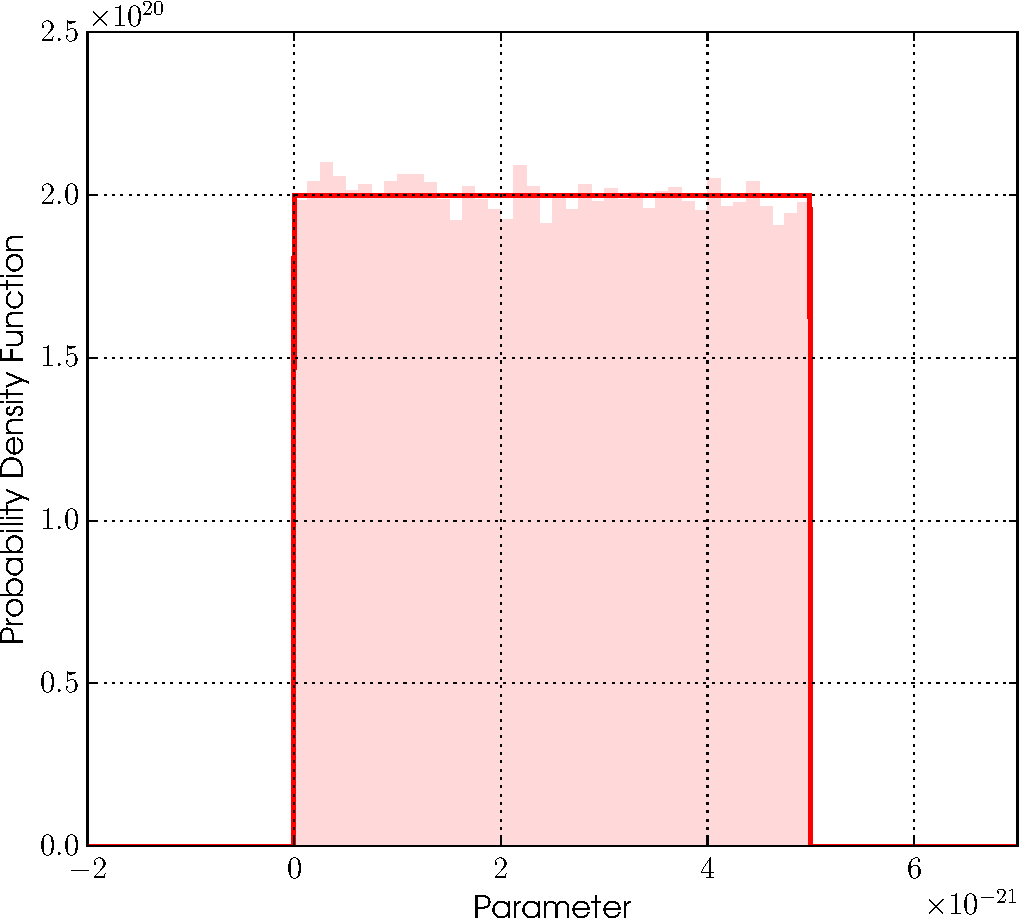
\includegraphics[width=1\columnwidth]{./figures/priors/uniform/uniform}
\caption{ \protect\label{fig:prioruniform}
Histogrammed samples drawn from the uniform prior distribution (solid line).
}
\end{center}
\end{figure}

\subsubsection{Gaussian prior}\label{sec:gaussianprior}

A parameter can be given a prior with a Gaussian distribution, defined by its mean, $\mu_x$, and standard deviation, $\sigma_x$, i.e.\
\begin{equation}
 p(x|I) = \frac{1}{\sqrt{2\pi\sigma_x^2}}\exp{\left[-\frac{(x-\mu_x)^2}{2\sigma_x^2}\right]}.
\end{equation}

A histogram of a set of samples produced by the code when drawing from a Gaussian prior distribution are shown in Figure~\ref{fig:priorgaussian},
along with the true prior function.

As well as single parameters being given Gaussian priors, we can define a set of $k$ parameters, $\vec{x}$, to have a multi-variate Gaussian prior
\begin{equation}
 p(\vec{x}|I) = \frac{\exp{\left(-\frac{1}{2}[\vec{x}-\vec{\mu_x}]'C^{-1}[\vec{x}-\vec{\mu_x}] \right)}}{(2\pi)^{k/2}|C|^{1/2}},
\end{equation}
where $\vec{\mu_x}$ are the means and $C$ is the covariance matrix. In reality we input the correlation coefficient matrix and individual
parameter standard deviations rather than the covariance matrix, but it is easy to convert between the two.

\begin{figure}[!phtb]
\begin{center}
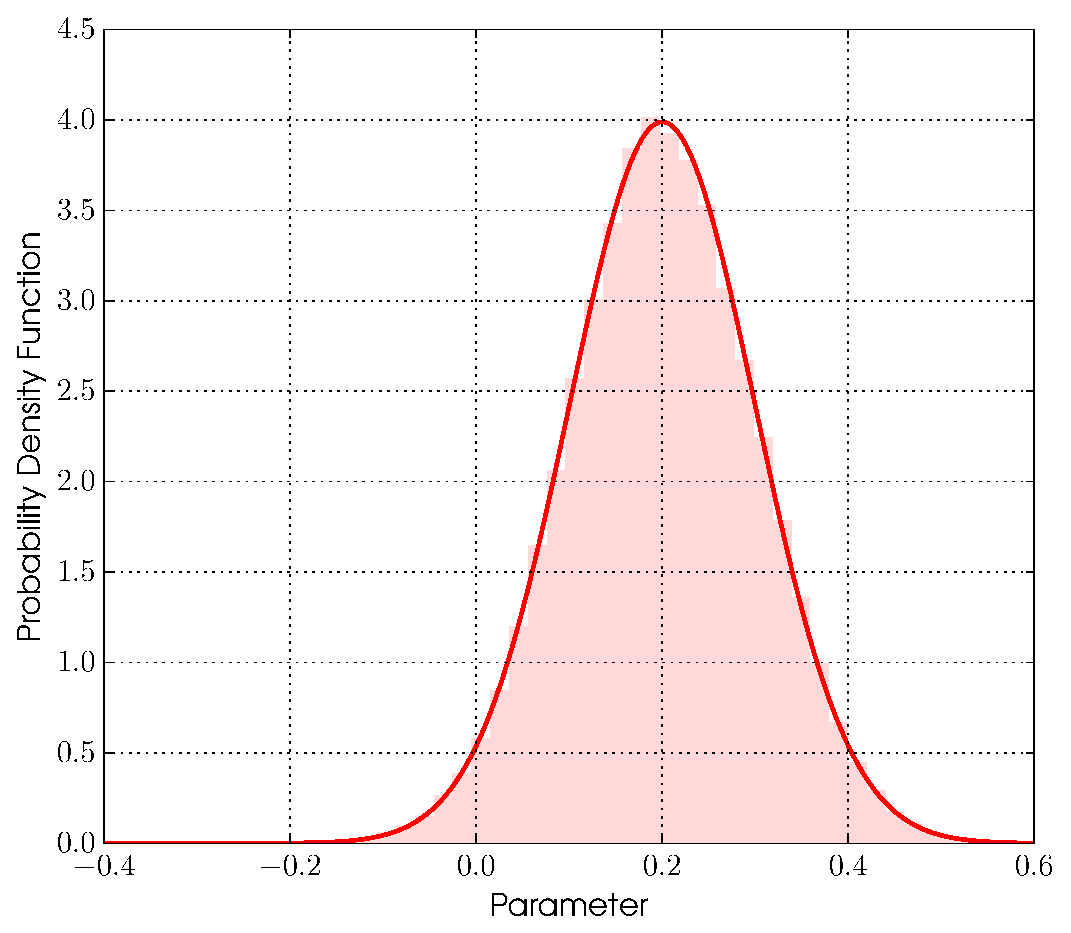
\includegraphics[width=1\columnwidth]{./figures/priors/gaussian/gaussian}
\caption{ \protect\label{fig:priorgaussian}
Histogrammed samples drawn from the Gaussian prior distribution (solid line).
}
\end{center}
\end{figure}

\subsubsection{Gaussian Mixture Model prior}\label{sec:gmmprior}

A parameter, or any set of parameters, can be given a prior distribution composed of a superposition of Gaussian distributions (a
Gaussian Mixture Model), with each component defined by a set of means for each parameter, a covariance matrix, and a weight
describing the relative probability concentrated in it. For an $n$ component mixture on a set of $k$ parameters, $\vec{x}$, the prior
function will be
\begin{equation}
 p(\vec{x}|I) = \sum_{i=1}^n w_i\frac{\exp{\left(-\frac{1}{2}{\Delta\vec{x}_i}'C_i^{-1}\Delta\vec{x}_i\right)}}{(2\pi)^{k/2}|C_i|^{1/2}},
\end{equation}
where, for component $i$, $w_i$ is the weight, $\Delta\vec{x_i}= \vec{x}-\vec{\mu}_{x_i}$, $\vec{\mu}_{x_i}$ are the means, and
$C_i$ is the covariance matrix.

Such a model can be used, for example, if there is a bimodal Gaussian prior on a particular parameter, as is the case for the
inclination angle $\iota$ if it is calculated from fits to pulsar wind nebulae \citep[see, e.g., Appendix B in][]{2017arXiv170107709T}. In such a case the Gaussian Mixture Model can define
two Gaussian distributions of equal standard deviations and weights. A more complex use of this prior would be for creating a smooth
probability distribution using samples drawn from it, i.e.\ taking posterior samples from a search for a particular pulsar, and
creating a smooth model of those samples (for, say, the two parameters $h_0$ and $\cos{\iota}$) to be input as a prior when looking
at future data for the same source.

Two examples of histograms of samples drawn from one-dimensional Gaussian Mixture Models with two and three modes respectively
are shown in Figure~\ref{fig:priorgmm}.

\begin{figure}[!phtb]
\begin{center}
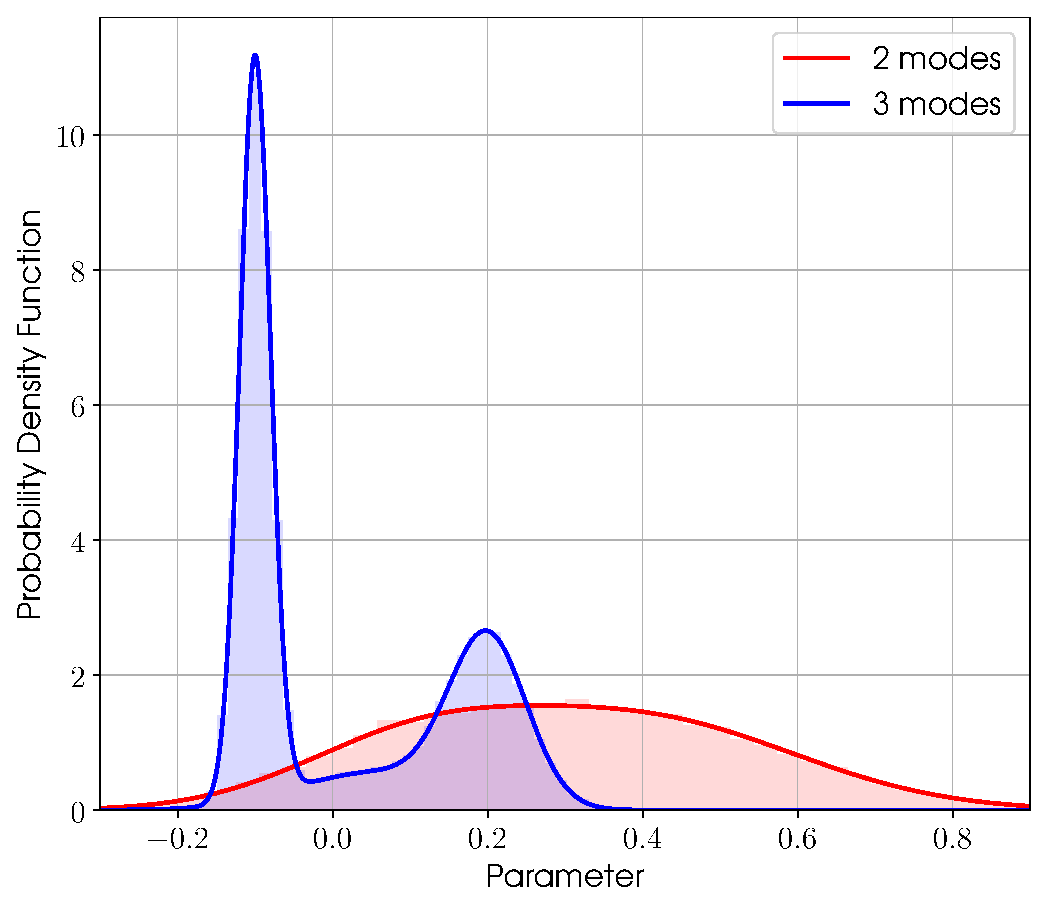
\includegraphics[width=1\columnwidth]{./figures/priors/gmm/gmm}
\caption{ \protect\label{fig:priorgmm}
Histogrammed samples drawn from two different Gaussian mixture model prior distributions (solid lines).
}
\end{center}
\end{figure}

\subsubsection{Log-Uniform prior}\label{sec:loguniform}

A parameter can be given a prior distribution that is uniform in the logarithm of the parameter, i.e.
\begin{equation}
 p(x|I) = \begin{cases}
             \left(\ln{x_{\text{max}}}-\ln{x_{\text{min}}}\right)^{-1}\frac{1}{x} & \text{if } x_{\text{min}} < x < x_{\text{max}}, \\
             0 & \text{otherwise}.
            \end{cases}
\end{equation}
This prior requires minimum and maximum values to be specified to make it normalisable and allow samples to be drawn from the
distribution. It should be noted that the choice of range, and in particular the lower bound, can have a significant effect on
the calculated evidence \citep[see, e.g., Appendix~B of][]{MaxCWpolariations}.

A histogram of a set of samples produced by the code when drawing from a log-uniform prior distribution, with a range between
$10^{-3}$ and 1 are shown in Figure~\ref{fig:priorloguniform}, along with the true prior function.

\begin{figure}[!phtb]
\begin{center}
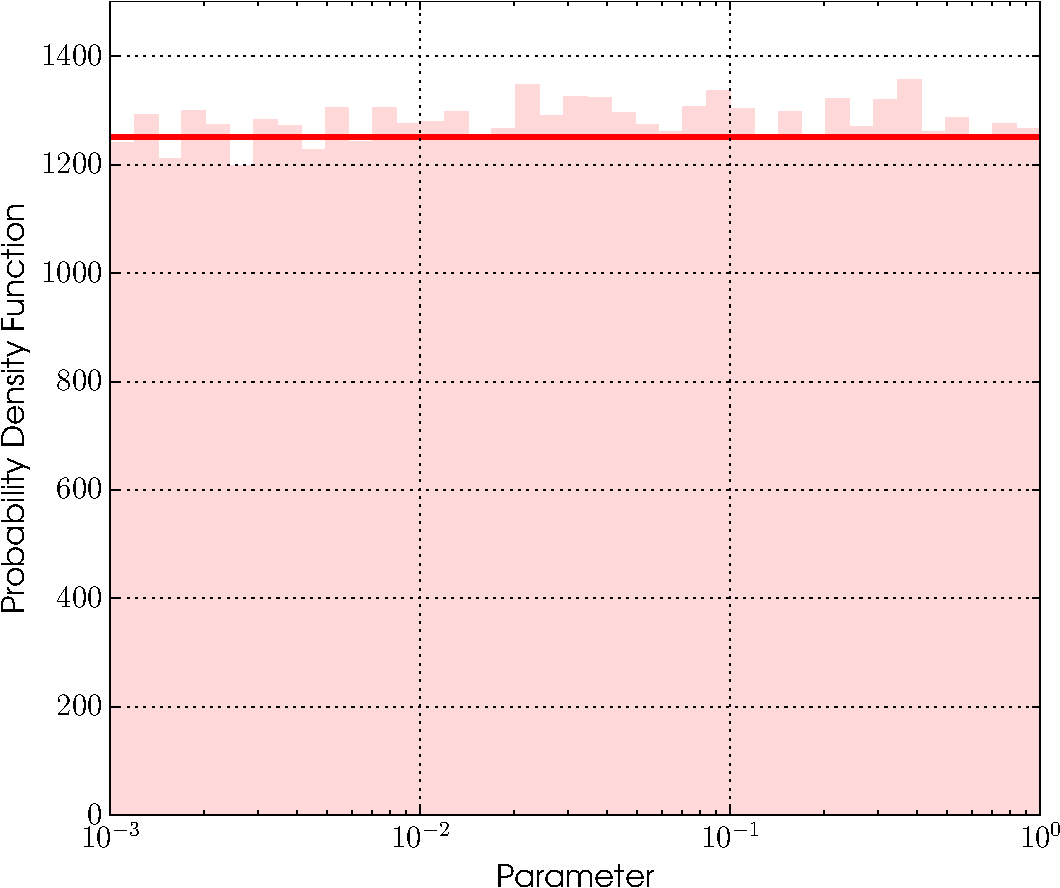
\includegraphics[width=1\columnwidth]{./figures/priors/loguniform/loguniform}
\caption{ \protect\label{fig:priorloguniform}
Histogrammed samples drawn from the log-uniform prior distribution (solid line).
}
\end{center}
\end{figure}

\subsubsection{Fermi-Dirac prior}\label{sec:fdprior}

A Fermi-Dirac distribution prior function was inspired by that used in \citet{Middleton_2015}. The prior has a sigmoid, or logistic,
shape, although starts at large values and slopes downwards and is restricted to positive values. The form of the function, for
parameter $x$, is
\begin{equation}\label{eq:fermidirac}
 p(x|\sigma, \mu, I) = \begin{cases}\frac{1}{\sigma\ln{\left(1+e^{\mu/\sigma} \right)}}\left(e^{(x-\mu)/\sigma} + 1\right)^{-1} & \text{if } x \geqslant 0, \\
                        0 & \text{otherwise},
                       \end{cases}
\end{equation}
and is defined by two parameters $\sigma$ and $\mu$. $\mu$ defines the point at which the distribution falls to 50\% of
its maximum value, whilst $\sigma$ defines the range over which the attenuation happens. We also make use of a parameter
$r = \mu/\sigma$. The band over which the probability falls from 97.5\% to 2.5\% of its maximum value is given by $\mu \pm Z\mu/2r$, where
$Z\approx7.33$. Therefore, if we want, for example, the distribution to have this particular fall-off over a range that is 10\% of $\mu$,
we would have $Z/2r = 0.1$ and $\sigma = 0.027\mu$.

Three different examples of Fermi-Dirac priors, and samples drawn from them by the code, are shown in Figure~\ref{fig:priorfermidirac},
for a selection of $\mu$ and $\sigma$ values.

\begin{figure}[!phtb]
\begin{center}
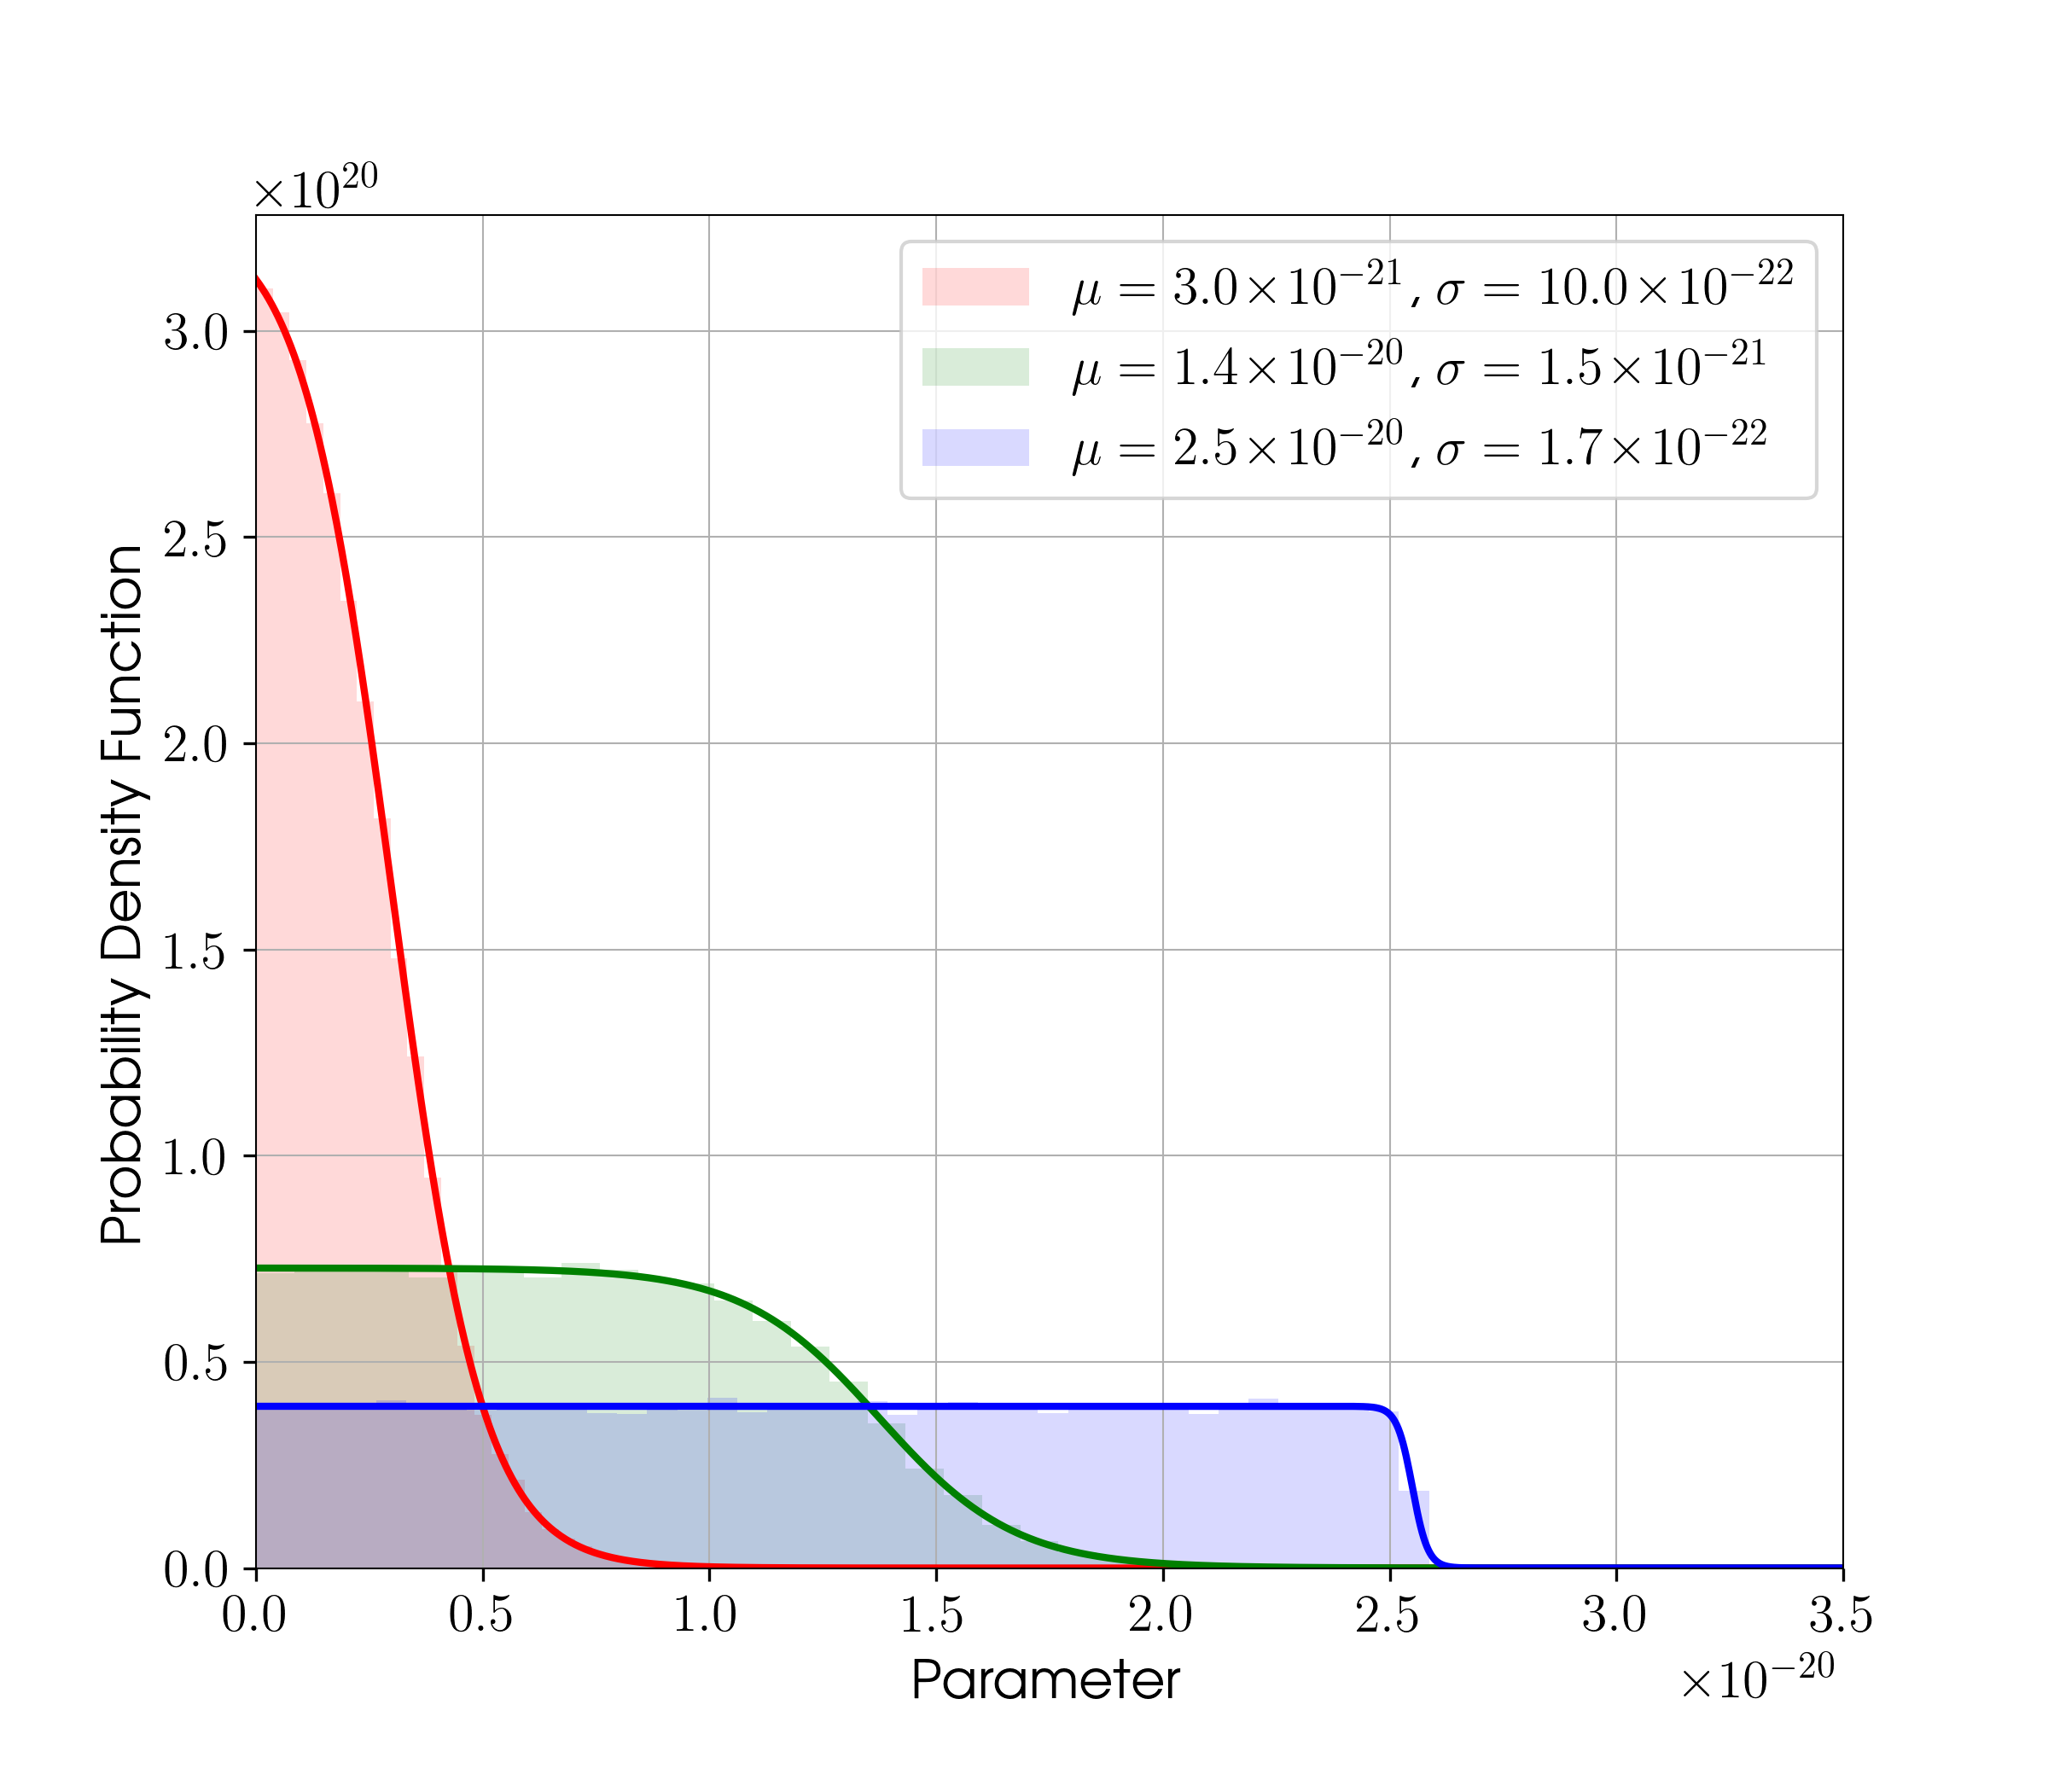
\includegraphics[width=1\columnwidth]{./figures/priors/fermidirac/fermidirac}
\caption{ \protect\label{fig:priorfermidirac}
Histogrammed samples drawn from three Fermi-Dirac prior distributions (solid lines), with the given $\mu$ and $\sigma$ values.
}
\end{center}
\end{figure}

The sampling from the prior uses inverse transform sampling. The cumulative distribution function (CDF) of Equation~\ref{eq:fermidirac}
is
\begin{widetext}
\begin{align}
 C(X_0) &= \int_0^{X_0} \frac{1}{\sigma\ln{\left(1+e^{r} \right)}}\left(e^{(x-\mu)/\sigma} + 1\right)^{-1} \text{d}x, \nonumber \\
 &= \frac{1}{\ln{\left(1+e^{r}\right)}}\left[\frac{X_0}{\sigma} + \ln{\left(1+e^{-r} \right)} - \ln{\left( 1+e^{(X_0-\mu)/\sigma}\right)} \right],
\end{align}
which can be inverted to give
\begin{equation}
X_0 = -\sigma \ln{}\left(-e^{-r} + \left(1+e^{r} \right)^{-C(X_0)} + e^{1-r}\left(1+e^{r} \right)^{-C(X_0)} \right).
\end{equation}
\end{widetext}
Thus, drawing CDF samples uniformly between 0 and 1, and inverting via the above equation gives values drawn from Equation~\ref{eq:fermidirac}.

This prior can use useful for amplitude parameters, where a uniform prior may have previously been used. It has the property of being roughly
flat at low values of the parameter and with an exponential fall-off at large values. This gives the advantage over a uniform prior with a
sharp upper cut-off in that the distribution is continuous rather than (perhaps) arbitrarily truncated.

This form of prior was used for the \gw amplitude parameter, $h_0$, in \citet{2017arXiv170107709T} as opposed to the earlier use of
a uniform prior with arbitrary upper cut-off used in, e.g., \citet{2014ApJ...785..119A}.

\subsection{Splitting the data}\label{sec:splitting}

The Student's $t$-likelihood function (\S\ref{sec:stlikelihood}) requires us to have an idea about the timescales on which the data is
stationary, i.e.\ periods when the noise in the data is best described as being drawn from a single
Gaussian distribution. We therefore use a scheme similar to the BayesianBlocks change point algorithm
\citep{1998ApJ...504..405S}, or BlockNormal \gw burst finding algorithm \citep{2004CQGra..21S1705M}, to find points at which the statistics of the
noise changes. This is done with a top-down iterative {\it divide and conquer} approach \citep{2000physics...9033S}.

We start by taking a full complex time series data set for a detector and subtracting a running median from both
the real and imaginary components. This
subtraction is performed to try and remove the effect of any very strong signals in the data, as we want to
assess the properties of the noise rather than any signal.\footnote{In reality this is only likely to be a current issue for strong
simulated signals injected into the data, as real signals will most likely have a low signal-to-noise ratio in short stretches of data.} The running median is calculated over a running window
of 30 data points (or a minimum of 15 points at the start are end of the data), but not accounting for gaps in the data.
For the standard data sample rate of
1 per 60 seconds, this means that half an hour of data is used, over which time the detector antenna patterns will not change
too drastically (unless there is a gap in the data). However, it should be noted that if using much more slowly sampled data set
then this hardcoded 30 sample window may not work well for very strong signals.

The next thing we do is calculate the evidence that the whole (running-median-removed) dataset is drawn from a single
Gaussian distribution with unknown variance. To do this we just use Equation~\ref{eq:nulllike}, with $N_{\text{dets}} =1$,
$N_{\text{s}}=1$, $M_{1,1}=1$, $n_{1,1,0}=1$ and, given a dataset of length $N$, set $m_{1,1,1}=N$. We will call the natural logarithm
of this value $\ln{\mathcal{Z}_{\text{single}}}$. We want to calculate the odds between this evidence and that for the data containing
{\it any} single change point (i.e. point at which the data seems to be drawn from a different Gaussian distribution). So, for
one single change point, at index $i$, we calculate $\ln{\mathcal{Z}_{\text{cp,i}}}$, by using Equation~\ref{eq:nulllike} and setting
$N_{\text{dets}} =1$, $N_{\text{s}}=1$, $M_{1,1}=2$, $n_{1,1}=\{1,i\}$ and $m_{1,1} = \{i,N-i\}$. We also impose a minimum allowed data
chunk size of $n_{\text{min}}$ (which defaults to a value of 5 data points in the code), so that $i \geqslant n_{\text{min}}$. As we want
the evidence for {\it any} single change point, we must take the sum all the single change point evidences
\begin{equation}
 \ln{\mathcal{Z}_{\text{any-cp}}} = \ln{\left(\sum_{i=n_{\text{min}}}^{N-n_{\text{min}}} \mathcal{Z}_{\text{cp,i}} \right)}.
\end{equation}
Finally, we are left with the odds (assuming equal prior probabilities for each hypothesis)
\begin{equation}\label{eq:cpodds}
 \ln{\mathcal{O}_{\text{any-cp}}^{\text{single}}} = \ln{\mathcal{Z}_{\text{any-cp}}} - \ln{\mathcal{Z}_{\text{single}}},
\end{equation}
for which values above zero favour there being a change point in the data. We could simply use this as the criterion on which to
split the data into two chunks at the change point value $i$ with the largest evidence. However, in practice this leads to
data drawn from a single Gaussian distribution actually being split far too often, and also there being a dependence on the
data length. So, instead, we empirically calculate an odds threshold above which the value of Equation~\ref{eq:cpodds} must be to
impose a split in the data.\footnote{A different approach would be to apply different priors to each hypothesis, although we have just taken
the empirical approach.} The empirical threshold we use is worked out by finding the 99\% upper limit on the value of
Equation~\ref{eq:cpodds} when data is purely drawn from a single Gaussian distribution (i.e. it gives a 1\% false alarm probability)
as a function of the data length $N$. The results of doing this for 30\,000 instances of data for a range of $n$ values, and three
different false alarm probabilities (1\%, 0.5\% and 0.1\%), are shown in Figure~\ref{fig:changepoint}. Fitting a line to the 1\% false alarm
probability points gives an odds ratio threshold dependence of
\begin{equation}
 T = 4.07 + 1.33\log{}_{10}{N}.
\end{equation}

\begin{figure}[!phtb]
\begin{center}
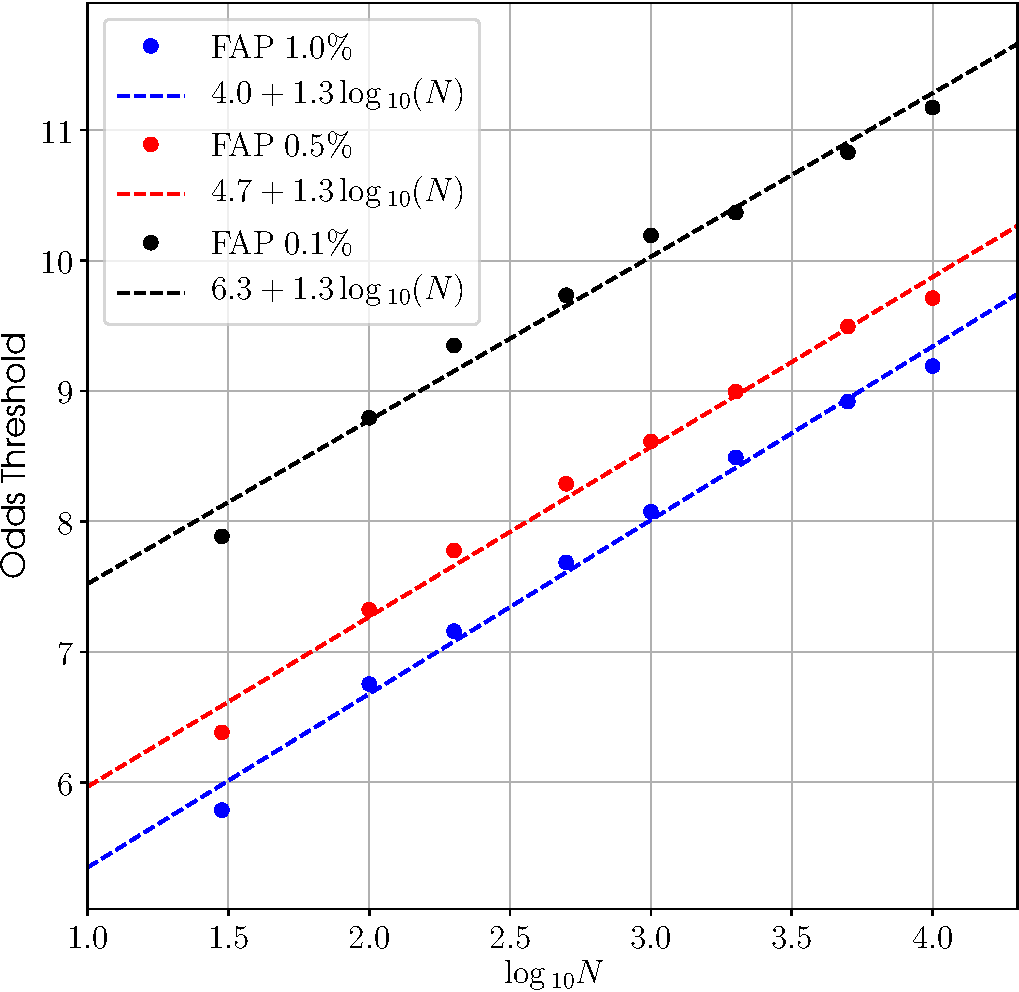
\includegraphics[width=1\columnwidth]{./figures/changepoint/changepoint}
\caption{ \protect\label{fig:changepoint}
The odds threshold as a function of data length for three different false alarm probabilities (FAP) calculated for
multiple realisations of simulated Gaussian noise. 
}
\end{center}
\end{figure}

The above process just splits the data once, so it must be applied iteratively to split the data further. When a change point is
found then the process is repeated on the two split data chunks, and stops when either no change point is found within a chunk,
or the split would give a segment smaller than $n_{\text{min}}$.

\subsection{Signal-to-noise ratio calculation}\label{sec:snr}

Whether a signal is found or not, the code will generate a signal-to-noise ratio (SNR). The calculated SNR uses the set of signal
parameters, $\vec{\theta}_{\text{ML}}$, that give the maximum value for the likelihood, which are then used to create the best-fit
complex signal template $y(\vec{\theta}_{\text{ML}})$. We then use calculations of the
noise standard deviation for each data chunk after removal of a running median from the data (the splitting and running median are
described in \S\ref{sec:splitting}). The {\it coherent} SNR is then calculated as
\begin{equation}\label{eq:snr}
 \rho_{\text{coh}} = \sqrt{\sum_{i=1}^{N_{\text{dets}}} \sum_{j=1}^{N_{\text{s}}}
\sum_{k=1}^{M_{i,j}} \sum_{n=n_{i,j,0}}^{n_{i,j,0}+(m_{i,j,k}-1)}\left(\frac{|y(\vec{\theta}_{\text{ML}})_{i,j,n}|^2}{\sigma_{i,j,k}^2}\right)},
\end{equation}
using the notation given in \S\ref{sec:likelihood}.\footnote{If using data input from the spectral interpolation code \citep{2017CQGra..34a5010D}
the noise standard deviations are actually passed to the code (see \S\ref{app:examples}), so in Equation~\ref{eq:snr} $M_{i,j}$ is replaced
by $L_{i,j}$ and $y(\vec{\theta}_{\text{ML}})_{i,j,n}$ is replace by $y(\vec{\theta}_{\text{ML}})_{i,j,k}$ as in \S\ref{sec:glikelihood}.}

A plot of the residual between the recovered single-detector and joint detector SNRs and their true values versus the true signal SNRs,
as calculated from Equation~\ref{eq:snr}, for a set of simulated signals (described in \S\ref{sec:simsignal}) are shown in Figure~\ref{fig:snrplot}.
The standard deviation of the resisduals is found to be one, with a mean around zero, and does not appear to change as a function of SNR (except at the
lowest SNRs, where the noise in the data will generally give rise to a maximum likelihood model with a larger amplitude than the true signal, and this
an overestimate of the SNR).

\begin{figure}[!phtb]
\begin{center}
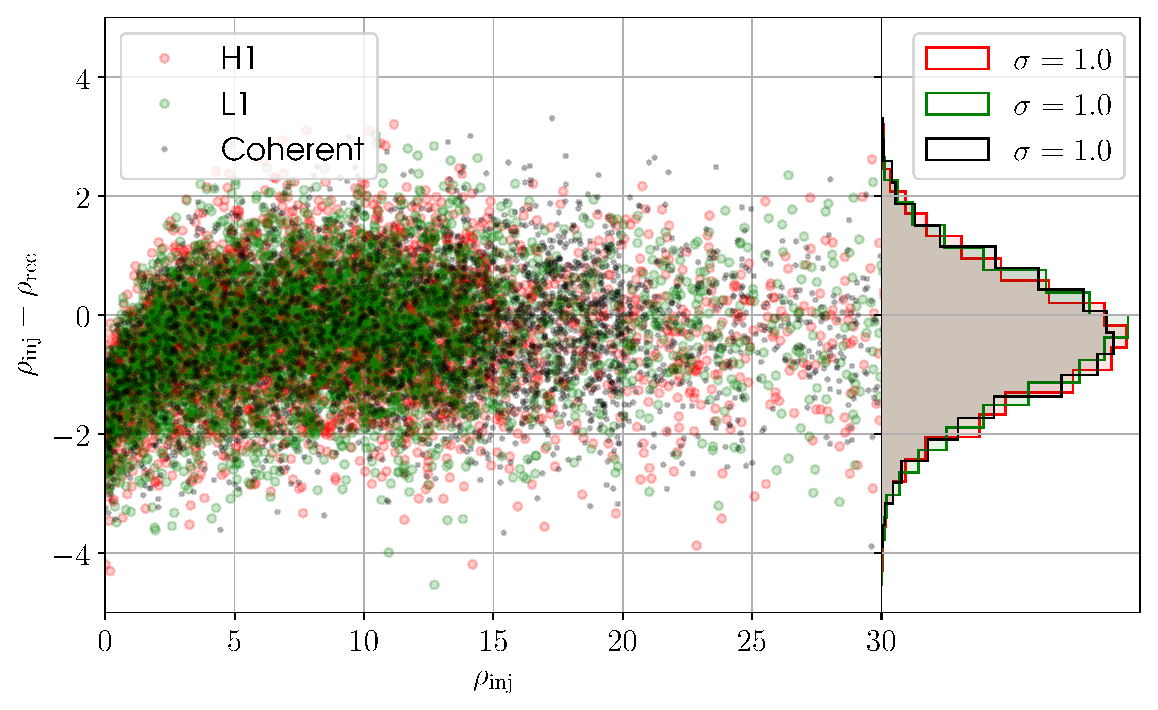
\includegraphics[width=1\columnwidth]{./figures/codeeval/stats/snrs/snr_plot}
\caption{ \protect\label{fig:walkpropks}
A set of violin plots showing the distributions of Kolmogorov-Smirnov test
two-sided $p$-values comparing the posterior sample CDFs with the analytical
CDFs as a function of the prior range, when using only the ensemble walk proposal distribution. The different colour plot represent different numbers of live points used.
Offsets around the different prior range values are just used to avoid overlaps of the
distributions.
}
\end{center}
\end{figure}

\subsection{Odds values}\label{sec:odds}

This is not explicitly a core function of the code, but here we will define some model selections (odds between competing models)
\begin{equation}
 \mathcal{O}_{M_1/M_2} = \frac{\mathcal{Z}_{M_1}}{\mathcal{Z}_{M_2}}\frac{p(M_1|I)}{p(M_2|I)},
\end{equation}
that can be produced from the output of the code. The code outputs two (natural logarithm) evidence values: the evidence for a coherent signal
($\mathcal{Z}_{\text{S}}$)
in all the datastreams (multi-detector and multi-frequency-band), and the evidence ($\mathcal{Z}_{\text{noise}}$) for the data consisting of
Gaussian noise (in sets of stationary segments as described in \S\ref{sec:splitting}). These can be combined in various ways for different model
selection situations, and we will define three such situations here \citep[see, e.g.,][for two of these]{2017arXiv170107709T}:
\begin{enumerate}
 \item the odds for a (multi-detector and multi-frequency-band) coherent signal versus (non-stationary) Gaussian noise, $\mathcal{O}_{\text{S}/\text{N}}$;
 \item the odds for a (multi-detector and multi-frequency-band) coherent signal versus incoherent (between detector) signals, $\mathcal{O}_{\text{S}/\text{I}_{\text{simple}}}$;
 \item the odds for a (multi-detector and multi-frequency-band) coherent signal versus combinations of incoherent (between detector) signals or noise,
 $\mathcal{O}_{\text{S}/\text{I}}$ \citep[cf.\ Equation~A6 in][]{2017arXiv170107709T}.
\end{enumerate}

The first of these (actually also given in Equation~\ref{eq:oddsratio}) just requires the two evidence values, $\mathcal{Z}_{\text{S}}$ and $\mathcal{Z}_{\text{noise}}$
\begin{align}\label{eq:sigvsnoise}
 \mathcal{O}_{\text{S}/\text{N}} &= \frac{\mathcal{Z}_{\text{S}}}{\mathcal{Z}_{\text{noise}}}, \nonumber \\
 \ln{\left(\mathcal{O}_{\text{S}/\text{N}}\right)} &= \ln{\left(\mathcal{Z}_{\text{S}}\right)} - \ln{\left({\mathcal{Z}_{\text{noise}}}\right)}.
\end{align}
The second requires that the code has been run for a multi-detector analysis, and also individually for each detector, $i$, to give $\mathcal{Z}_{\text{S}_i}$
and $\mathcal{Z}_{\text{N}_i}$, and is given by
\begin{align}\label{eq:cohvincoh1}
 \mathcal{O}_{\text{S}/\text{I}_{\text{simple}}} &= \frac{\mathcal{Z}_{\text{S}}}{\prod_i^{N_{\text{dets}}} \mathcal{Z}_{\text{S}_i}}, \nonumber \\
 \ln{\left(\mathcal{O}_{\text{S}/\text{I}_{\text{simple}}}\right)} &= \ln{\left(\mathcal{Z}_{\text{S}}\right)} - \sum_i^{N_{\text{dets}}}\ln{\left(\mathcal{Z}_{\text{S}_i}\right)}.
\end{align}
Such an odds is useful in vetoing strong incoherent signals that are therefore not astrophysical, e.g.\ instrumental lines \citep[see, e.g., the similar
line-robust statistic defined in][]{2014PhRvD..89f4023K}. In both these cases it is assumed
that the prior odds ($p(M_1|I)/p(M_2|I)$) between the two models are set to be equal and therefore are not explicitly given.

The third odds makes use of a compound model in the denominator with all evidences for all permutations of Gaussian noise or incoherent signal being used.
If we have the set of single detector signal and Gaussian noise models $M_j = \{\text{S}_j, \text{N}_j\}$, then \citep[see, e.g., Equation~50 of][]{MaxCWpolariations}
\begin{equation}\label{eq:cohvincoh2}
 \mathcal{O}_{\text{S}/\text{I}} = \frac{\mathcal{Z}_{\text{S}}p(\text{S}|I)}{\prod_{j=1}^{N_{\text{dets}}}\left[ Z_{\text{S}_j}p(\text{S}_j|I) + Z_{\text{N}_j}p(\text{N}_j|I) \right]},
\end{equation}
where $p(\text{S}|I)$ is the prior on the coherent signal model, and $p(\text{S/N}_j|I)$ are the priors for the signal/noise hypotheses for each individual detector.
As there are two possible models for data in each detector, signal or noise, the number of logical {\it or} combined sub-hypotheses \citep[see, e.g., the four sub-hypotheses
used in Equation~A6 of][where the priors in the denominator are the combinations that would be given from expanding out equation~\ref{eq:cohvincoh2}]{2017arXiv170107709T}
in the compound model is just given by $2^{N_{\text{dets}}}$. In \citet{2017arXiv170107709T}, and later in this 
document, we have assigned the equal probabilities to the coherent signal prior
and to each of the sub-hypothesis priors in the denominator, so that they cancel out. However, other priors could be used.

It is also worth noting that in all the above cases the models (and sub-hypotheses) are mutually exclusive. This may not at first seem obvious, as,
for example, the Gaussian noise model is contained within the signal model provided the prior on the signal amplitude allowed a value of zero. But, as noted in
\citet{2012PhRvD..85h2003L, MaxCWpolariations}, within the signal noise hypothesis having an amplitude of exactly zero (as in the Gaussian
noise hypothesis) occupies an infinitesimally thin slice of the parameter space, and therefore has no weight. The same can be said for the a coherent
signal within the incoherent signal model.
